\chapter{PCG Techniques}
The most important thing to keep in mind when working with PCG is that different environments require different PCG methods. Before we start looking specifically into dungeon generation we must first identify the major PCG techniques to decide which one fits best.

\section{Genetic algorithms}
Togelius et al. distinguishes two types of content generation. The first is with the use of a {\em constructive algorithm} that consists of generating the content in a single run with little or no backtracking \citep{springerlink:10.1007/togelius1}. The other method, referred to as {\em generate-and-test algorithms}, carries out a number of attempts and select only the candidates that satisfy a set of tests \citep{springerlink:10.1007/togelius1}. Typically, such algorithms are more complicated and more time-consuming, however if handled with care they can provide results in only a fraction of a second \citep{DBLP:conf/cig/TogeliusPBWHY10}. Due to the nature of genetic algorithms, they tend to provide very good results for generating outdoor terrain or, in other words, generating the height-map of a level \citep{DBLP:conf/gecco/RaffeZL11}.

Genetic algorithms are essentially generate-and-test algorithms \citep{springerlink:10.1007/togelius1}. A genetic algorithm can metaphorically be described as:
\begin{quote}
``Genetic Algorithms mimic real life evolution, in particular based on Darwin’s theory of Natural Selection" ... ``Features change over time due to natural mutations and mutual heritance." \citep{DBLP:conf/ACMace/MouratoSB11}.
\end{quote}

The idea of a genetic algorithm is to create a series of candidates, selectively pick out the best ones and then repeat this process until a satisfactory solution emerges \citep{DBLP:conf/ACMace/MouratoSB11}.

\begin{figure}[h!]
  \centering
    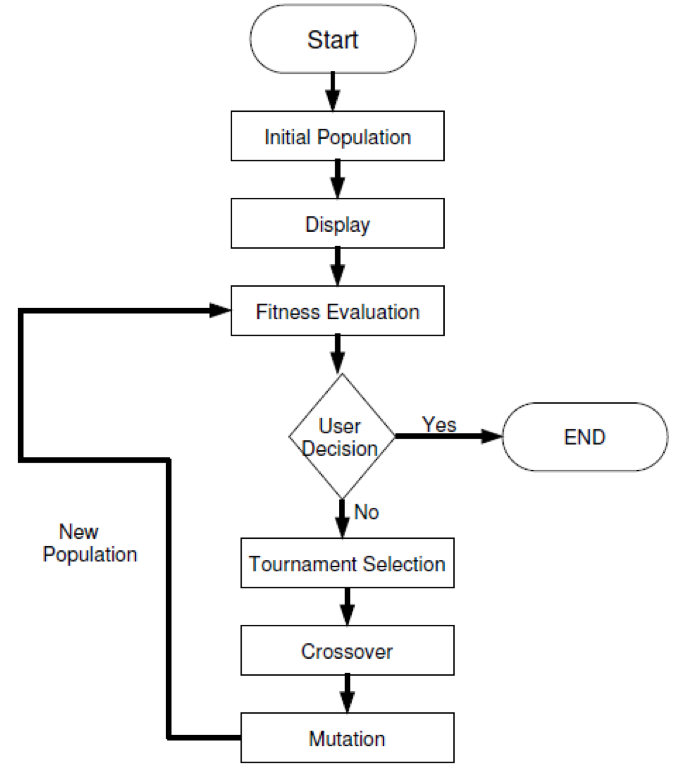
\includegraphics[width=0.4\textwidth]{images/genetic-flowchart.png}
\caption{Flowchart representation of a genetic algorithm. Image sourced from \citep{DBLP:conf/cec/WalshG10}}
\end{figure}

\subsection{Fitness function}
The key element in any genetic algorithm is the {\em fitness function}, which is the function that defines `how good' a solution is. This function is used to test the validity of a candidate \citep{DBLP:conf/evoW/SorensonP10}. 

Based on the usage of this fitness function, we can obtain entirely different results. Sorenson and Pasquier demonstrated that it is possible to conceive a generic framework for PCG by considering the fitness function as the amount of fun a level can convey. Naturally, the concept of fun is a rather abstract concept from a mathematical point of view. Their fitness function is dependant on a challenge measurement function, which is specific to a certain genre of game. This abstraction on the fitness function allows the algorithm to generate content both for a 2D side-scrolling platform game (such as {\em Super Mario Brothers}) as well for a dungeon-like top-down view game (such as {\em The Legend of Zelda}) \citep{DBLP:conf/evoW/SorensonP10}.

The fitness function can measure anything based on what is required. For instance, using a fitness function that measures fun is probably more viable for creating the environment of a video game \citep{DBLP:conf/evoW/SorensonP10}, whereas a function that measures the aesthetics of a terrain is more suited if the algorithm is intended to generate beautiful terrain \citep{DBLP:conf/cec/WalshG11}.

\subsection{Genetic operators}
When candidates are selected they will evolve in some way. Raffe et al. distinguish two kinds of selections: {\em parent selection} and {\em gene selection} \citep{DBLP:conf/gecco/RaffeZL11}. Distinguishing between the two is not necessary, but in doing so one gets an increased amount of control on how the algorithm behaves \citep{DBLP:conf/gecco/RaffeZL11}.

\paragraph{Mutation} This is where a single candidate evolves on its own, meaning certain genes will change into different values. The mutation can be random or selective \citep{DBLP:conf/ACMace/MouratoSB11}.
\paragraph{Cross-over} This is where two candidates are mixed together. How these two candidates are mixed depends on the type of problem being solved and the desired result \citep{DBLP:conf/ACMace/MouratoSB11}.

\section{Search-Based}
Search-based content generators are based around viewing the generation process as a search problem with a starting state, a goal state and several randomised intermediate states. They can be used to generate different kinds of content depending on how the algorithm is used. According to Togelius et al., Search-based procedural content generation (SBPCG) algorithms are generally based upon some sort of evolutionary algorithm \citep{DBLP:conf/cig/TogeliusPBWHY10}.

Togelius et al. define a search-based algorithm as such:
\begin{quote}
``Search-based procedural content generation (SBPCG) is a particular type of generate-and-test PCG, where the generated candidate content is not simply rejected or accepted by the test but graded on one or several numeric dimensions, and where a search algorithm is used to find better content based on the evaluations of previously generated content."\citep{DBLP:conf/cig/TogeliusPBWHY10}
\end{quote}

A SBPCG algorithm was used by Togelius et al. to procedurally generate maps for the Real-time strategy game StarCraft. These maps are generated by using in-game objectives such as mineral fields and geysers as the goals of the search-problem \citep{DBLP:conf/cig/TogeliusPBWHY10}.

However, search-based procedural generation techniques can also be used for generating random maze-like structures using a method suggested by Ashlock et al. This method used an algorithm that consists of visiting parts of the maze at random using a fitness function. An interesting feature about this method is that it's independent from the representation of the maze. The authors demonstrate the execution on three kinds of representations \citep{DBLP:journals/tciaig/AshlockLM11} :
\begin{itemize}
\item {\bf Direct:} Represented by a grid where each element is a bit that represents either a wall, by the value 1, or a walk-able area, by the value 0.
\item {\bf Indirect positive:} Values are stored in an array and represent the walls of the maze.
\item {\bf Indirect negative:} Values are stored in an array and represent the empty space (rooms and corridors) of the maze.
\end{itemize}
Naturally all these representation can be expanded to include more possible values and, in doing so, allow different kinds of terrain / walls across the maze \citep{DBLP:journals/cim/AshlockLM11}.

Ashlock et al. also clearly illustrate the importance of the fitness function. Here are some examples of different results obtain by merely using a different function \citep{DBLP:journals/tciaig/AshlockLM11}:
\begin{itemize}
\item {\bf Exit Path Length Fitness ($F_1$):} The function causes the maze to be composed of a single long path.
\item {\bf Primitive Re-convergence Sum Fitness ($F_2$):} This can produces a maze with dead-ends, also referred to as cul-de-sacs.
\item {\bf Isolated Primary Re-convergence Sum Fitness ($F_3$):} This function produces a maze with paths that split off and meet up again at the end.
\end{itemize}

\begin{figure}[h!]
  \centering
    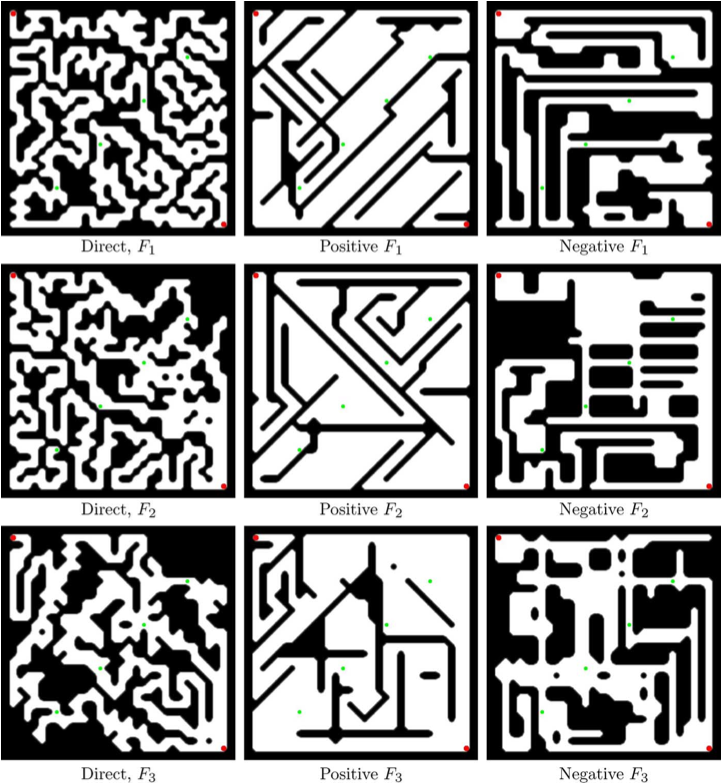
\includegraphics[width=0.50\textwidth]{images/ashlockMazes.png}
  \caption{An illustration of the various types of mazes generated \citep{DBLP:journals/tciaig/AshlockLM11}.}
\end{figure}


\section{Rhythm-Based} 
In platform-genre video games such as {\em Super Mario} and so forth, the aspect of timing and rhythm is particularly important \citep{DBLP:journals/tciaig/SmithWMTMC11}. Such games revolve around the fact that the player must hit the right keys at the right time. One example of timing is the act of running and jumping to get across a gap in the level. If the player jumps too early, they will not reach the next platform and fall. If the player presses the jump button too late then their character would fall before starting the jump \citep{Smith:2008:FAP:1401843.1401858}.

\begin{figure}[h!]
  \centering
    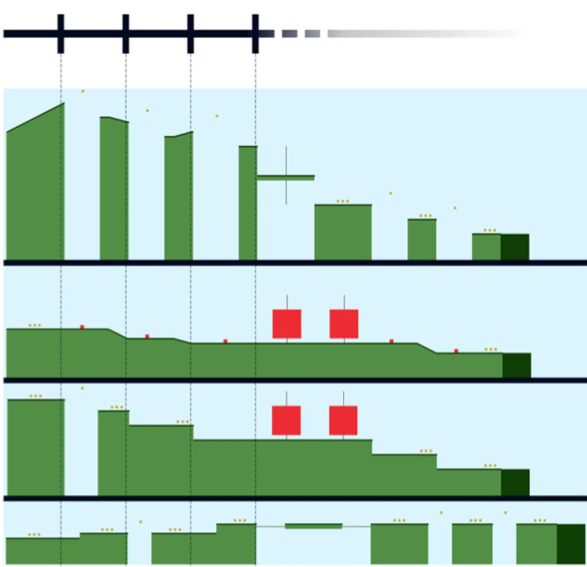
\includegraphics[width=0.28\textwidth]{images/rhythm.png}
  \caption{Platform game level generation using a rhythm-based technique \citep{DBLP:journals/tciaig/SmithWMTMC11}}
\end{figure}

A level generator called Launchpad has been designed based on this key concept of rhythm \citep{DBLP:journals/tciaig/SmithWMTMC11}.
The generator creates sections that are either `jump' or `walk'. The frequency of these jumps is defined by the rhythm of the algorithm. Additionally the length and height of the terrain will vary at random \citep{DBLP:journals/tciaig/SmithWMTMC11}. 

N. Shaker et al. then conceived an optimisation to such an algorithm using Artificial Intelligence (AI) \citep{DBLP:conf/aiide/ShakerYT10}. The algorithm consists of first generating a level at random. Afterwards, an AI player plays through the level and the action's of that player are recorded. Based on these actions the algorithm will then optimise the level to make it more enjoyable.

Needless to say, such algorithms are directed specifically to platform games and are not directly applicable to other genres. Although these algorithms are aimed at 2D games a 3D implementation could still be possible but would involve a large increase of constraints.


\section{Occupancy-regulated}
The main disadvantage with purely randomised levels is that things can look a little bit unnatural or lack the sense of creativity. Human-designed levels present the advantage of being more unique and more suited to the type of game developed \citep{DBLP:conf/cig/MawhorterM10}. Mawhorter and Mateas have suggested an occupancy-regulated algorithm that allows random levels to be used whilst maintaining liberty and control for human level designer.

The authors summarise the algorithm as such:
\begin{quote}
``Occupancy-regulated extension works by assembling a level using chunks from a library." \citep{DBLP:conf/cig/MawhorterM10}.
\end{quote}

\begin{figure}[h!]
  \centering
    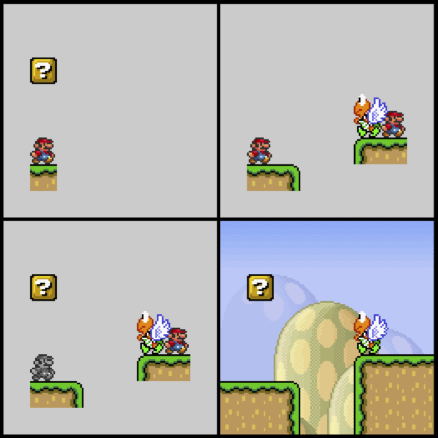
\includegraphics[width=0.35\textwidth]{images/mario.png}
  \caption{An illustration of Mawhorter and Mateas' algorithm. The two top panels are individual chunks. The lower left panel presents the two chunks mixed. The lower right panel is the result after post-processing. Image source: \citep{DBLP:conf/cig/MawhorterM10}}
\end{figure}


The idea is that level designers need only to design small key sections of the level that are referred to as `chunks'. Each chunk consists primarily of empty space along with certain aspects of the game, such as a jump, an NPC spawn point and so forth. Along with this, each chunk has a set of pre-defined locations where the players can legally situate themselves. These locations are called anchors \citep{DBLP:conf/cig/MawhorterM10}.

The algorithm then uses these anchors to blend several chunks together. It will take one anchor from each chunk and maps those anchors to the same location in the world. Once the level is complete the post-processor will fill the empty areas with additional components such as decorations and un-passable terrain. \citep{DBLP:conf/cig/MawhorterM10}.

This method can produce some very interesting and enjoyable levels but can cause a lot of repetition if the chunk-library is too small \citep{DBLP:conf/cig/MawhorterM10}. For example, players of the game title Diablo 3 will notice a lot of identical rooms being repeated. This suggests that this title uses some kind of occupancy-regulated algorithm, although there is no real evidence to support this.


\section{Procedural Modelling}
Procedural modelling is special kind of PCG in which the algorithm generates a 3D mesh. Algorithms that we have explored until now focused on designing the structure of a maze, or the layout of platforms. However, none of these were particularly focused on the modelling aspect of an environment.

In an article published in 2003 the authors present an interesting way of procedurally modelling skyscrapers in real-time \citep{DBLP:conf/graphite/GreuterPSL03}. The method consists of building the floor-plan by piling primitive shapes on one another and obtaining the union of that region \citep{DBLP:conf/graphite/GreuterPSL03}. The border of this floor-plan is then extruded to form a 3D object and this process is repeated for the succeeding stories \citep{DBLP:conf/graphite/GreuterPSL03}. This method is a simple, elegant and a cost-efficient way of procedurally modelling a random room. A method like this could be used to generate the rooms of a dungeon.

Procedural modelling can used also be done using L-systems. Parish and M\"uller suggested a method of using extended L-systems to generate the road map in the form of a graph. They then use L-systems again to procedurally construct the geometry of the buildings. The authors also propose a method of procedurally generating the textures of the meshes, which effectively causes a wider range of building styles to be generated \citep{Parish:2001:PMC:383259.383292}.

\begin{figure}[h!]
  \centering
    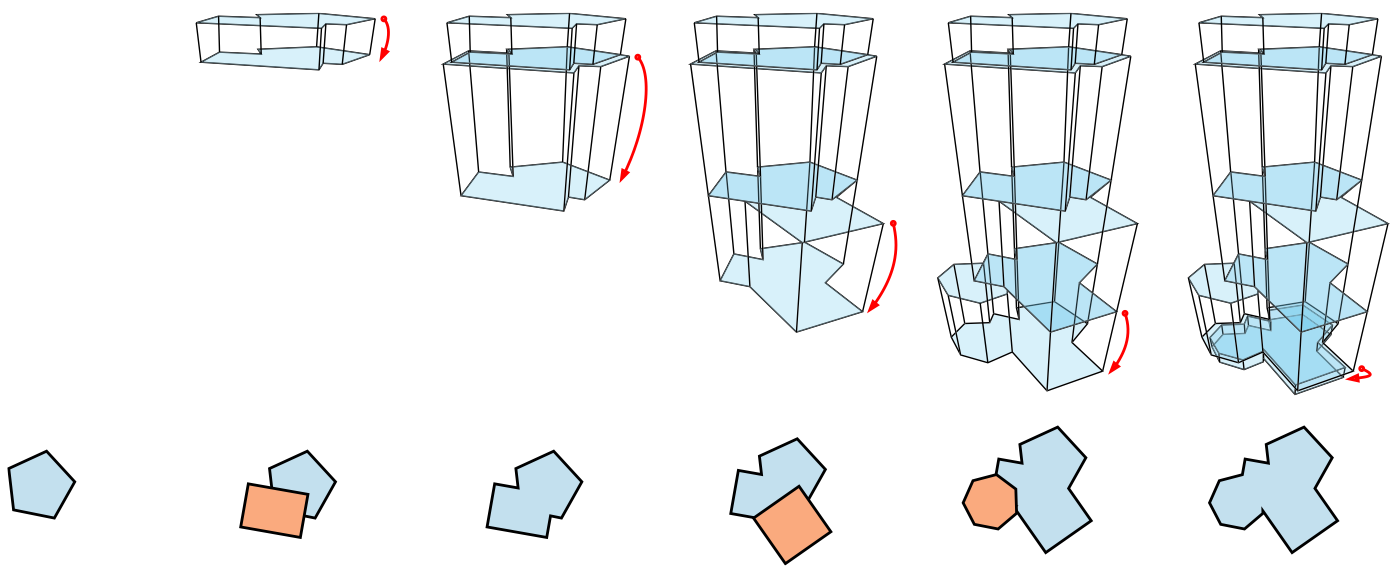
\includegraphics[width=0.75\textwidth]{images/floorplan.png}
  \caption{The various steps of the floor-plan generation. Image source: \citep{DBLP:conf/graphite/GreuterPSL03}}
\end{figure}

Another interesting topic is how to interconnect structures together through bridges, staircases and so forth. One simple approach to link two structures together is by simply interconnecting them linearly using a shape such as a box for instance \citep{DBLP:journals/cgf/KrecklauK11}. However this may not always look convincing and is not sufficient to generate interconnections with curves and deformed pieces \citep{DBLP:journals/cgf/KrecklauK11}. 

Various methods exist to generate non-linear interconnections. One example is to use a rigid chain, a structure which is best described as a:
\begin{quote}
``sequence of revolute (rotational) and prismatic (translational) joints." \citep{DBLP:journals/cgf/KrecklauK11}
\end{quote}
The angles and positions of these joints can be calculated through the use of Inverse Kinematics (IK) \citep{DBLP:journals/cgf/KrecklauK11}. However when solving an IK problem a solution may not always exist, such as if the target point is out of arm's reach \citep{Tolani2000353}. A good IK solving algorithm must not only be able to find a solution if one exists, but it should also detect and report if a result is unreliable or no solution could be found \citep{Tolani2000353}.

Hahn et al. have developed a method to generate the interior content of a building with multiple floors in real-time. It uses lazy execution to insure that content is only generated once the player approaches a portal near an un-explored region. They use a number of strict generation rules to follow when generating content in order to do so efficiently. The algorithm uses a {\em generation tree} to divide the large space into floor divisions, hallway divisions, and room cluster division \citep{Hahn:2006:PRB:1183316.1183342}.